\documentclass[12pt,a4paper]{article}
\usepackage[utf8]{inputenc}
\usepackage{amsmath,amssymb,amsthm}
\usepackage{graphicx}
\usepackage{hyperref}
\usepackage{geometry}
\usepackage{booktabs}
\usepackage{algorithm}
\usepackage{algpseudocode}
\usepackage{tikz}
\usepackage{physics}
\usepackage{siunitx}
\usepackage{subcaption}

\geometry{margin=1in}

\newtheorem{theorem}{Theorem}[section]
\newtheorem{lemma}[theorem]{Lemma}
\newtheorem{proposition}[theorem]{Proposition}
\newtheorem{corollary}[theorem]{Corollary}
\newtheorem{definition}[theorem]{Definition}

\title{Refraction Puzzle Imaging: Discrete Light Propagation as Combinatorial Constraint Satisfaction at Planck-Adjacent Temporal Resolution}

\author{Kundai Farai Sachikonye}

\date{2025}

\begin{document}

\maketitle

\begin{abstract}
We introduce Refraction Puzzle Imaging (RPI), a theoretical framework that recasts optical image formation as a discrete combinatorial constraint satisfaction problem. By operating at temporal precision approaching $10^{-156}$~s---far exceeding conventional timescales---light propagation becomes effectively discretized into finite steps of approximately $10^{-148}$~m. At this resolution, each photon trajectory through an optical system constitutes a sequence of categorical state transitions governed by discretized Snell's law. Image reconstruction transforms from continuous wave optics into solving a finite constraint satisfaction problem where detected intensity patterns constrain the space of valid source configurations. We develop the mathematical framework for this discretization, derive the state transition algebra for common optical elements, and analyze computational complexity bounds. Application to fluorescence microscopy, phase contrast imaging, optical coherence tomography, and scattering media demonstrates that RPI enables theoretical reconstruction of images from arbitrarily aberrated or scattered light fields. We establish conditions under which the inverse problem admits unique solutions and characterize the information-theoretic limits of the approach.
\end{abstract}

\section{Introduction}

Conventional optical imaging operates in the wave-optical regime where light is treated as continuous electromagnetic fields governed by Maxwell's equations. Image formation is understood through diffraction theory, with resolution fundamentally limited by the Abbe criterion \cite{Abbe1873}. While super-resolution techniques have pushed beyond this limit \cite{Hell1994,Betzig2006,Gustafsson2000}, they operate within the same continuous wave paradigm.

We propose a radical departure: treating light propagation as a discrete combinatorial process. This approach becomes physically meaningful at temporal precision of order $10^{-156}$~s, where light traverses distances of approximately $10^{-148}$~m per temporal unit. At this scale, photon trajectories decompose into finite sequences of discrete steps, and optical phenomena such as refraction become categorical state transitions rather than continuous field transformations.

The key insight is that image reconstruction---traditionally an inverse problem in continuous wave optics---becomes a constraint satisfaction problem (CSP) over finite discrete states. A detected image represents constraints on source configurations, and reconstructing the original scene is equivalent to finding assignments that satisfy these constraints.

This paper develops the theoretical foundations for Refraction Puzzle Imaging (RPI) and analyzes its application across multiple microscopy modalities.

\subsection{Motivation: The Discretization Threshold}

Consider light propagating through a medium with refractive index $n$. The phase velocity is:
\begin{equation}
v = \frac{c}{n}
\end{equation}

At temporal resolution $\delta t$, light traverses a spatial step:
\begin{equation}
\delta x = \frac{c \cdot \delta t}{n}
\end{equation}

For $\delta t \sim 10^{-156}$~s and $n \sim 1$, we obtain $\delta x \sim 3 \times 10^{-148}$~m. This scale is vastly smaller than any physical structure---smaller than the Planck length ($\ell_P \sim 10^{-35}$~m) by 113 orders of magnitude.

However, the physical relevance emerges not from measuring at this scale, but from the \emph{combinatorial finiteness} it induces. For any finite optical system of size $L$ and duration $T$, the number of possible photon trajectories becomes:
\begin{equation}
N_{\text{paths}} \leq \left(\frac{L}{\delta x}\right)^3 \cdot \frac{T}{\delta t}
\end{equation}

For a $\SI{100}{\micro\meter}$ sample observed over $\SI{1}{\femto\second}$, this yields approximately $10^{450}$ possible paths---enormous but \emph{finite}. The transition from infinite continuous trajectories to finite discrete paths enables fundamentally different computational approaches.

\section{Mathematical Framework}

\subsection{Discrete State Space}

\begin{definition}[Photon State]
A photon state at temporal index $\tau$ is a tuple:
\begin{equation}
\ket{\psi_\tau} = (\mathbf{r}_\tau, \mathbf{k}_\tau, \phi_\tau, \sigma_\tau)
\end{equation}
where $\mathbf{r}_\tau \in \mathcal{L}$ is the discretized position on lattice $\mathcal{L}$, $\mathbf{k}_\tau$ is the discretized wavevector, $\phi_\tau \in [0, 2\pi)_d$ is the discretized phase, and $\sigma_\tau \in \{+, -\}$ denotes polarization.
\end{definition}

The lattice $\mathcal{L}$ is defined with spacing $\delta x$ over the optical volume. Wavevectors are similarly discretized with angular resolution $\delta\theta$ determined by the lattice structure.

\begin{definition}[Transition Operator]
A transition operator $\hat{T}$ maps states between consecutive temporal indices:
\begin{equation}
\hat{T}: \ket{\psi_\tau} \mapsto \ket{\psi_{\tau+1}}
\end{equation}
The operator encodes the local optical properties at position $\mathbf{r}_\tau$.
\end{definition}

\subsection{Discretized Snell's Law}

At an interface between media with refractive indices $n_1$ and $n_2$, Snell's law becomes a categorical state transition. Let $\theta_1$ be the incident angle (discretized) and $\theta_2$ the refracted angle.

\begin{theorem}[Discrete Snell Transition]
The refraction transition $\hat{T}_{\text{Snell}}$ satisfies:
\begin{equation}
\theta_2 = \text{round}\left(\arcsin\left(\frac{n_1}{n_2} \sin\theta_1\right), \delta\theta\right)
\end{equation}
where $\text{round}(\cdot, \delta\theta)$ projects to the nearest discrete angle on the lattice.
\end{theorem}

The discretization introduces a fundamental granularity. For angles where $\frac{n_1}{n_2} \sin\theta_1 > 1$, total internal reflection occurs as a categorical switch rather than continuous transition.

\begin{definition}[Interface Transition Matrix]
For an interface with discretized angles $\{\theta_j\}_{j=1}^{N_\theta}$, the transition matrix $\mathbf{M}_{\text{int}}$ has elements:
\begin{equation}
M_{jk} = \begin{cases}
|t_{jk}|^2 & \text{if } \theta_k = \hat{T}_{\text{Snell}}(\theta_j) \\
|r_{jk}|^2 & \text{if } \theta_k = -\theta_j \text{ (reflection)} \\
0 & \text{otherwise}
\end{cases}
\end{equation}
where $t_{jk}$ and $r_{jk}$ are Fresnel coefficients.
\end{definition}

\subsection{Free Propagation as Lattice Walk}

Between optical elements, photons execute a constrained lattice walk. Given current state $(\mathbf{r}, \mathbf{k})$, the next position is:
\begin{equation}
\mathbf{r}' = \mathbf{r} + \delta x \cdot \hat{\mathbf{k}}
\end{equation}
where $\hat{\mathbf{k}}$ is the unit direction vector, discretized to lattice directions.

\begin{proposition}[Walk Constraint]
The number of lattice directions $N_d$ in 3D is bounded by:
\begin{equation}
N_d \leq \frac{4\pi}{(\delta\theta)^2}
\end{equation}
For practical discretization with $\delta\theta \sim 10^{-3}$ radians, $N_d \sim 10^7$ directions.
\end{proposition}

\subsection{Phase Accumulation}

Phase accumulates discretely:
\begin{equation}
\phi_{\tau+1} = \phi_\tau + k \cdot n(\mathbf{r}_\tau) \cdot \delta x \mod 2\pi
\end{equation}

The discretized phase $\phi \in \{0, \delta\phi, 2\delta\phi, \ldots, 2\pi - \delta\phi\}$ with $\delta\phi = 2\pi/N_\phi$ for integer $N_\phi$ introduces quantization of interference effects.

\section{Image Formation as Constraint Satisfaction}

\subsection{The Forward Problem}

Consider an optical system with source distribution $S(\mathbf{r})$ and detector array $D(\mathbf{r}')$. The forward model computes detected intensities:
\begin{equation}
I(\mathbf{r}') = \sum_{\text{paths } p: S \to \mathbf{r}'} w(p) \cdot S(\mathbf{r}_p^{\text{source}})
\end{equation}
where $w(p)$ encodes path attenuation and phase factors.

In the discrete framework, paths are finite sequences of states:
\begin{equation}
p = (\ket{\psi_0}, \ket{\psi_1}, \ldots, \ket{\psi_N})
\end{equation}
with $\ket{\psi_N}$ terminating at detector position $\mathbf{r}'$.

\begin{definition}[Path Weight]
The weight of path $p$ is:
\begin{equation}
w(p) = \prod_{\tau=0}^{N-1} T(\psi_\tau \to \psi_{\tau+1}) \cdot e^{i\Phi(p)}
\end{equation}
where $T(\cdot \to \cdot)$ is the transition amplitude and $\Phi(p) = \sum_\tau \phi_\tau$ is the accumulated phase.
\end{definition}

\subsection{The Inverse Problem as CSP}

\begin{theorem}[RPI Reconstruction]
Given detected intensities $\{I(\mathbf{r}'_j)\}_{j=1}^M$ at $M$ detector positions, reconstructing source distribution $S$ is equivalent to finding an assignment to discrete source variables $\{s_i\}_{i=1}^{N_s}$ satisfying:
\begin{equation}
\sum_{i=1}^{N_s} A_{ji} \cdot s_i = I_j \quad \forall j \in \{1, \ldots, M\}
\end{equation}
where $A_{ji} = \sum_{\text{paths } p: i \to j} w(p)$ is the path-sum transfer coefficient from source voxel $i$ to detector pixel $j$.
\end{theorem}

\begin{proof}
The discretization ensures $A_{ji}$ is well-defined as a finite sum over the finite path space. The inverse problem reduces to solving the linear system $\mathbf{A}\mathbf{s} = \mathbf{I}$.
\end{proof}

The key insight is that $\mathbf{A}$ is computable---in principle---by exhaustive enumeration of discrete paths. While computationally intractable in naive form, the structure admits efficient algorithms.

\subsection{Uniqueness Conditions}

\begin{theorem}[Reconstruction Uniqueness]
The RPI inverse problem has unique solution if and only if:
\begin{enumerate}
    \item $\text{rank}(\mathbf{A}) = N_s$ (full column rank)
    \item The system is not underdetermined: $M \geq N_s$
\end{enumerate}
\end{theorem}

In practice, uniqueness depends on the optical geometry. Aberrations that appear catastrophic in wave optics may actually \emph{increase} rank by coupling additional spatial modes.

\begin{corollary}[Scattering Enhancement]
For scattering media where paths diverge chaotically, the transfer matrix $\mathbf{A}$ generically achieves full rank, guaranteeing unique reconstruction.
\end{corollary}

This counterintuitive result---that scattering aids rather than hinders imaging---is a distinctive prediction of the RPI framework.

\section{Application to Microscopy Modalities}

\subsection{Fluorescence Microscopy}

In fluorescence microscopy, emitters at positions $\{\mathbf{r}_i\}$ produce incoherent intensity:
\begin{equation}
I_{\text{fl}}(\mathbf{r}') = \sum_i c_i \cdot |G(\mathbf{r}', \mathbf{r}_i)|^2
\end{equation}
where $c_i$ is emitter brightness and $G$ is the Green's function.

\subsubsection{Discrete Green's Function}

In the RPI framework, the Green's function becomes:
\begin{equation}
G_{\text{disc}}(\mathbf{r}', \mathbf{r}) = \sum_{\text{paths } p: \mathbf{r} \to \mathbf{r}'} w(p)
\end{equation}

For well-corrected optics, paths concentrate along classical ray trajectories. For aberrated systems, path weights spread across configuration space.

\begin{proposition}[Aberration Invariance]
Under RPI, aberrated and unaberrated systems differ only in path weight distribution, not in reconstructability. If the transfer matrix remains full rank, perfect reconstruction is possible.
\end{proposition}

This implies that aberration correction becomes unnecessary---aberrations are computationally inverted rather than optically corrected.

\subsubsection{Single-Molecule Localization}

For single-molecule localization microscopy (SMLM), individual emitters produce isolated PSFs. RPI enables:

\begin{equation}
\mathbf{r}_{\text{true}} = \argmin_{\mathbf{r}} \left\| I_{\text{detected}} - |G_{\text{disc}}(\cdot, \mathbf{r})|^2 \right\|^2
\end{equation}

The discrete path structure provides exact localization bounded only by photon statistics, not optical aberrations.

\subsection{Phase Contrast and Quantitative Phase Imaging}

Phase contrast microscopy converts optical path length differences into intensity variations. The standard model uses:
\begin{equation}
I_{\text{PC}} = I_0 \left[1 + 2\phi \sin\beta + \phi^2\right]
\end{equation}
where $\phi$ is phase shift and $\beta$ is the phase ring retardation.

\subsubsection{Discrete Phase Recovery}

In RPI, phase is discretized: $\phi \in \{k\delta\phi\}_{k=0}^{N_\phi-1}$. The inverse problem becomes:

\begin{theorem}[Phase Quantization Theorem]
For phase contrast with discretization $\delta\phi$, the maximum recoverable optical path difference is:
\begin{equation}
\text{OPD}_{\max} = \frac{\lambda N_\phi}{2\pi}
\end{equation}
Phase unwrapping is automatically resolved by the discrete constraint structure.
\end{theorem}

The discretization eliminates phase wrapping ambiguities inherent in continuous phase imaging.

\subsection{Optical Coherence Tomography}

OCT measures depth-resolved reflectivity through low-coherence interferometry:
\begin{equation}
I_{\text{OCT}}(z) = \int R(z') \cdot \Gamma(z - z') dz'
\end{equation}
where $R(z)$ is sample reflectivity and $\Gamma$ is the coherence function.

\subsubsection{Discrete Depth Sampling}

RPI discretizes depth as $z_k = k\delta z$. The coherence function becomes:
\begin{equation}
\Gamma_{\text{disc}}(z_j - z_k) = \sum_{\text{paths}} w(p) \cdot \delta_{\text{coherent}}(p)
\end{equation}
where $\delta_{\text{coherent}}$ enforces coherence gating through path length matching.

\begin{proposition}[Axial Resolution Enhancement]
The discrete path formulation enables axial resolution:
\begin{equation}
\Delta z_{\text{RPI}} = \min\left(\Delta z_{\text{coherence}}, N_{\text{paths}}^{-1/3} \cdot L\right)
\end{equation}
where the second term represents the information-theoretic limit from path distinguishability.
\end{proposition}

For sufficient path diversity, this can exceed the coherence length limit of conventional OCT.

\subsection{Scattering Media: Diffuse Optical Imaging}

The most dramatic application is imaging through strongly scattering media where conventional optics fails entirely.

\subsubsection{Multiple Scattering as Path Branching}

In scattering media, photon paths branch at each scattering event:
\begin{equation}
\ket{\psi_\tau} \xrightarrow{\text{scatter}} \sum_{\theta,\phi} c_{\theta\phi} \ket{\psi_{\tau+1}(\theta,\phi)}
\end{equation}

The scattering function $c_{\theta\phi}$ is determined by particle properties (Mie theory, Rayleigh, etc.).

\begin{theorem}[Scattering Matrix Construction]
For a scattering medium with $N_s$ scatterers and $N_d$ discrete directions, the full scattering transfer matrix has dimension:
\begin{equation}
\dim(\mathbf{A}_{\text{scatter}}) = N_{\text{detector}} \times N_{\text{source}} \times N_s^{k_{\max}}
\end{equation}
where $k_{\max}$ is the maximum scattering order considered.
\end{theorem}

\subsubsection{Transmission Matrix Recovery}

The transmission matrix $\mathbf{T}$ relates input field $\mathbf{E}_{\text{in}}$ to output field $\mathbf{E}_{\text{out}}$:
\begin{equation}
\mathbf{E}_{\text{out}} = \mathbf{T} \cdot \mathbf{E}_{\text{in}}
\end{equation}

In RPI, $\mathbf{T}$ is constructed directly from path enumeration:
\begin{equation}
T_{jk} = \sum_{\text{paths } p: k \to j} w(p)
\end{equation}

Once $\mathbf{T}$ is known, imaging through scattering reduces to matrix inversion:
\begin{equation}
\mathbf{E}_{\text{source}} = \mathbf{T}^{-1} \cdot \mathbf{E}_{\text{detected}}
\end{equation}

\begin{corollary}[Generic Invertibility]
For random scattering media, $\mathbf{T}$ is generically invertible (full rank) with probability 1, enabling perfect image reconstruction.
\end{corollary}

\subsection{Super-Resolution Techniques}

\subsubsection{STED Microscopy in RPI Framework}

Stimulated emission depletion (STED) creates effective sub-diffraction PSFs through saturable transitions. In RPI:

\begin{equation}
G_{\text{STED}}(\mathbf{r}', \mathbf{r}) = G_{\text{exc}}(\mathbf{r}', \mathbf{r}) \cdot \left[1 - \eta_{\text{STED}}(\mathbf{r})\right]
\end{equation}

where $\eta_{\text{STED}}$ is the depletion efficiency.

The discrete state space naturally represents the molecular states (ground, excited, depleted), and super-resolution emerges from the categorical structure of state transitions rather than wave-optical interference.

\subsubsection{Structured Illumination Microscopy}

SIM achieves resolution enhancement through pattern frequency mixing:
\begin{equation}
\tilde{I}_{\text{detected}}(\mathbf{k}) = \tilde{S}(\mathbf{k}) \otimes \tilde{H}(\mathbf{k}) \cdot \delta(\mathbf{k} - \mathbf{k}_{\text{pattern}})
\end{equation}

In RPI, the illumination pattern defines allowed source states:
\begin{equation}
s_i^{(n)} = s_i \cdot \cos(\mathbf{k}_n \cdot \mathbf{r}_i + \phi_n)
\end{equation}

Multiple pattern orientations provide constraint equations enabling sub-diffraction reconstruction.

\section{Computational Considerations}

\subsection{Complexity Analysis}

\begin{theorem}[Path Enumeration Complexity]
Naive enumeration of all discrete paths through an optical system of volume $V$, duration $T$, and discretization $\delta x$, $\delta t$ has complexity:
\begin{equation}
\mathcal{O}\left(N_d^{T/\delta t}\right)
\end{equation}
where $N_d$ is the number of discrete directions.
\end{theorem}

This is clearly intractable for macroscopic systems. However, physical constraints dramatically reduce the effective path space.

\subsection{Constraint Propagation}

\begin{proposition}[Causality Pruning]
Causality constraints eliminate all paths violating $|\mathbf{r}_{\tau+1} - \mathbf{r}_\tau| \leq c\delta t$, reducing path space by factor:
\begin{equation}
\frac{V_{\text{causal}}}{V_{\text{full}}} = \left(\frac{c\delta t}{\delta x}\right)^3
\end{equation}
\end{proposition}

\begin{proposition}[Optical Element Localization]
For systems with discrete optical elements (lenses, mirrors), paths are constrained to pass through element surfaces, enabling factorization:
\begin{equation}
\mathbf{A} = \mathbf{A}_{\text{det}} \cdot \mathbf{A}_{\text{elem}_n} \cdots \mathbf{A}_{\text{elem}_1} \cdot \mathbf{A}_{\text{source}}
\end{equation}
Complexity reduces to $\mathcal{O}(n \cdot N_{\text{elem}}^2)$ where $n$ is element count.
\end{proposition}

\subsection{Algorithm: Constrained Path Solver}

\begin{algorithm}[H]
\caption{RPI Reconstruction via Constrained Path Satisfaction}
\begin{algorithmic}[1]
\Require Detected intensities $\mathbf{I}$, optical system geometry $\mathcal{G}$, discretization $(\delta x, \delta t, \delta\theta)$
\Ensure Reconstructed source distribution $\mathbf{S}$

\State Initialize source lattice $\mathcal{L}_s$, detector lattice $\mathcal{L}_d$
\State Compute transition matrices for each optical element
\State $\mathbf{A} \gets$ Compose element matrices
\For{each detector pixel $j$}
    \State $\mathbf{A}[j,:] \gets$ Enumerate paths terminating at $j$
    \State Apply constraint propagation to prune infeasible paths
\EndFor
\If{$\text{rank}(\mathbf{A}) = |\mathcal{L}_s|$}
    \State $\mathbf{S} \gets \mathbf{A}^{-1} \mathbf{I}$ \Comment{Direct solution}
\Else
    \State $\mathbf{S} \gets$ Regularized least-squares solution
\EndIf
\State \Return $\mathbf{S}$
\end{algorithmic}
\end{algorithm}

\subsection{Iterative Refinement}

For large systems, iterative methods exploit sparsity:

\begin{equation}
\mathbf{S}^{(k+1)} = \mathbf{S}^{(k)} + \alpha \mathbf{A}^T (\mathbf{I} - \mathbf{A}\mathbf{S}^{(k)})
\end{equation}

The discrete structure enables integer programming relaxations and SAT solver integration for hard reconstruction problems.

\section{Information-Theoretic Limits}

\subsection{Channel Capacity}

The optical system viewed as communication channel has capacity:
\begin{equation}
C = \log_2 \left(\frac{N_{\text{source states}}}{N_{\text{ambiguity classes}}}\right)
\end{equation}

\begin{theorem}[RPI Channel Theorem]
For an optical system with transfer matrix $\mathbf{A}$:
\begin{equation}
C_{\text{RPI}} = \text{rank}(\mathbf{A}) \cdot \log_2(N_{\text{intensity levels}})
\end{equation}
\end{theorem}

Full-rank systems achieve channel capacity equal to the source dimensionality.

\subsection{Noise Bounds}

Photon shot noise imposes fundamental limits:
\begin{equation}
\text{SNR}_j = \sqrt{N_{\text{photons}}(j)}
\end{equation}

\begin{theorem}[Noise-Limited Resolution]
The minimum resolvable source feature size under photon noise is:
\begin{equation}
\delta_{\min} = \frac{\|\mathbf{A}^{-1}\|_2}{\sqrt{N_{\text{total photons}}}} \cdot \sigma_{\text{read}}
\end{equation}
where $\sigma_{\text{read}}$ is detector read noise.
\end{theorem}

\section{Experimental Considerations}

\subsection{Temporal Resolution Requirements}

Achieving $10^{-156}$~s resolution is beyond any foreseeable technology. However, the RPI framework provides value at much coarser discretization:

\begin{proposition}[Practical Discretization]
For wavelength $\lambda$ and desired spatial resolution $\Delta x$:
\begin{equation}
\delta t_{\text{practical}} = \frac{\Delta x}{c} \sim \frac{\lambda}{10c} \sim 10^{-16}~\text{s}
\end{equation}
Attosecond temporal resolution suffices for sub-wavelength spatial imaging.
\end{proposition}

Current technology achieves attosecond ($10^{-18}$~s) pulses \cite{Corkum2007}, placing practical RPI within reach.

\subsection{Measurement Protocol}

RPI requires:
\begin{enumerate}
    \item \textbf{Intensity measurement}: Standard detector arrays
    \item \textbf{System calibration}: Measuring $\mathbf{A}$ through point source scanning or wavefront sensing
    \item \textbf{Computational reconstruction}: Solving the inverse problem
\end{enumerate}

The calibration step is system-specific but needs to be performed only once for a given optical configuration.

\section{Intrinsic Spectral Decomposition}

A remarkable consequence of transplanckian temporal resolution is the automatic separation of light into its spectral components. At $10^{-156}$~s precision, we resolve timescales far finer than optical wave periods ($\sim 10^{-15}$~s), enabling wavelength-dependent path discrimination without external spectrometric apparatus.

\subsection{Chromatic Path Separation}

In any dispersive medium, the refractive index depends on wavelength through the Sellmeier relation:
\begin{equation}
n^2(\lambda) = 1 + \sum_i \frac{B_i \lambda^2}{\lambda^2 - C_i}
\end{equation}

At transplanckian resolution, photons of different wavelengths follow distinguishable discrete paths. The path velocity for wavelength $\lambda$ is:
\begin{equation}
v(\lambda) = \frac{c}{n(\lambda)}
\end{equation}

Over observation time $T$, wavelengths $\lambda_1$ and $\lambda_2$ accumulate a path difference:
\begin{equation}
\Delta x = c \left| \frac{1}{n(\lambda_1)} - \frac{1}{n(\lambda_2)} \right| T
\end{equation}

For this to be resolvable at spatial discretization $\delta x = c \cdot \delta t$:
\begin{equation}
\Delta x > \delta x \implies \left| \frac{1}{n(\lambda_1)} - \frac{1}{n(\lambda_2)} \right| > \frac{\delta t}{T}
\end{equation}

With $\delta t \sim 10^{-156}$~s and $T \sim 10^{-15}$~s (one optical cycle), even minute dispersion differences become resolvable.

\subsection{The Graduated Instrument}

The scattering medium itself functions as a \emph{graduated spectral analyzer}. Different wavelengths experience:

\begin{enumerate}
    \item \textbf{Different velocities}: UV travels slower than IR in most materials
    \item \textbf{Different scattering cross-sections}: Rayleigh scattering scales as $\lambda^{-4}$
    \item \textbf{Different penetration depths}: Absorption varies spectrally
    \item \textbf{Different transfer matrices}: Each $\lambda$ has its own $\mathbf{A}_\lambda$
\end{enumerate}

\begin{definition}[Spectral Transfer Tensor]
The full optical transfer becomes a tensor indexed by wavelength:
\begin{equation}
\mathcal{A}_{jk}^\lambda = \sum_{\text{paths } p: k \to j} w_\lambda(p)
\end{equation}
where path weights $w_\lambda(p)$ depend on wavelength through $n(\lambda)$, $\mu_s(\lambda)$, and $\mu_a(\lambda)$.
\end{definition}

\subsection{Hyperspectral Reconstruction}

The inverse problem naturally decomposes into wavelength-specific sub-problems:
\begin{equation}
\mathbf{I}_\lambda = \mathbf{A}_\lambda \cdot \mathbf{S}_\lambda \quad \forall \lambda \in \{\lambda_1, \ldots, \lambda_N\}
\end{equation}

\begin{theorem}[Spectral Separability]
At transplanckian resolution, the composite measurement $\mathbf{I}_{\text{total}} = \sum_\lambda \mathbf{I}_\lambda$ can be decomposed into spectral components if the transfer matrices $\{\mathbf{A}_\lambda\}$ are sufficiently distinct, i.e.:
\begin{equation}
\text{rank}\left( \begin{bmatrix} \mathbf{A}_{\lambda_1} \\ \vdots \\ \mathbf{A}_{\lambda_N} \end{bmatrix} \right) = \sum_\lambda \text{rank}(\mathbf{A}_\lambda)
\end{equation}
\end{theorem}

This implies that \textbf{hyperspectral imaging emerges for free} from the RPI framework---no spectrometer required.

\subsection{Wavelength-Dependent Scattering}

The scattering coefficient varies dramatically with wavelength:
\begin{equation}
\mu_s(\lambda) = \mu_{s,0} \left( \frac{\lambda_0}{\lambda} \right)^\alpha
\end{equation}
where $\alpha \approx 4$ for Rayleigh scattering (small particles) and $\alpha \approx 0.5$--$2$ for Mie scattering (larger structures).

\begin{table}[h]
\centering
\begin{tabular}{lccc}
\toprule
\textbf{Wavelength Band} & \textbf{n (typical)} & \textbf{$\mu_s$ (mm$^{-1}$)} & \textbf{Rank Enhancement} \\
\midrule
UV (300 nm) & 1.52 & 15.0 & High \\
Blue (450 nm) & 1.50 & 8.0 & High \\
Green (550 nm) & 1.49 & 5.5 & Medium \\
Red (650 nm) & 1.48 & 4.0 & Medium \\
NIR (800 nm) & 1.47 & 2.5 & Lower \\
IR (1000 nm) & 1.46 & 1.5 & Lower \\
\bottomrule
\end{tabular}
\caption{Wavelength-dependent optical properties in biological tissue. Higher scattering increases transfer matrix rank, improving reconstruction.}
\end{table}

The counterintuitive prediction from Section 4 (scattering enhances reconstruction) combines with spectral decomposition: \textbf{shorter wavelengths, which scatter more strongly, provide higher-rank transfer matrices and thus better reconstruction fidelity}.

\subsection{Implications for Cellular Imaging}

In cellular microscopy, different wavelengths probe different structural scales:
\begin{itemize}
    \item \textbf{UV (300--400 nm)}: Nucleic acids, aromatic amino acids
    \item \textbf{Visible (400--700 nm)}: Chromophores, fluorescent proteins
    \item \textbf{NIR (700--1000 nm)}: Water, lipids, deep tissue penetration
\end{itemize}

RPI automatically separates these contributions, enabling label-free hyperspectral cellular imaging through the intrinsic dispersion and scattering properties of biological matter.

\section{Partition Extraction: Tracing vs. Subtraction}

A fundamental reconceptualization emerges from the RPI framework: traditional image processing relies on \emph{subtraction} to isolate features, while RPI enables \emph{boundary tracing} that preserves total information.

\subsection{The Subtraction Paradigm and Its Limitations}

Conventional image processing follows a reductive pipeline:
\begin{equation}
L \xrightarrow{\text{subtract background}} L_1 \xrightarrow{\text{subtract noise}} L_2 \xrightarrow{\text{filter}} \cdots \xrightarrow{} L_{\text{final}}
\end{equation}

Each subtraction operation destroys information. For a sequence of $n$ operations with fidelity factors $\{f_i\}_{i=1}^n$ where $f_i < 1$:
\begin{equation}
\text{Information retained} = \prod_{i=1}^n f_i \ll 1
\end{equation}

This cascade of information loss is unavoidable in the subtraction paradigm---you cannot recover what has been removed.

\subsection{The Tracing Paradigm: Partition Extraction}

RPI introduces an alternative: rather than subtracting to isolate, we \emph{trace boundaries} to identify partitions within the complete field.

\begin{definition}[Partition Extraction]
Let $L$ be the total light field (complete path ensemble) and $P \subset L$ a region of interest. Partition extraction identifies the constraint set $\mathcal{C}$ such that:
\begin{equation}
P = \{p \in L : p \text{ satisfies } \mathcal{C}\}
\end{equation}
The boundary membrane $\partial P$ is the set of paths crossing the partition boundary.
\end{definition}

The crucial difference: \textbf{no information is removed from $L$}. The partition is identified by specifying which paths belong to it, not by discarding the rest.

\begin{theorem}[Information Preservation]
Partition extraction preserves total field information:
\begin{equation}
H(L) = H(P) + H(L \setminus P) + I(P; L \setminus P)
\end{equation}
where $H$ denotes entropy and $I$ denotes mutual information. The boundary $\partial P$ encodes the mutual information $I(P; L \setminus P)$.
\end{theorem}

\begin{proof}
The partition $(P, L \setminus P)$ is a refinement of $L$. Information decomposition follows from the chain rule for entropy. The boundary paths contribute to both $P$ and $L \setminus P$, encoding their relationship.
\end{proof}

\subsection{Holographic Extraction}

The boundary membrane $\partial P$ contains sufficient information to reconstruct the partition interior. This is a discrete analogue of the holographic principle.

\begin{definition}[Boundary Encoding]
The boundary encoding of partition $P$ is the constraint tuple:
\begin{equation}
\mathcal{E}(\partial P) = \left( \{p_{\text{cross}}\}, \{\theta_{\text{in/out}}\}, \{\phi_{\text{boundary}}\} \right)
\end{equation}
specifying crossing paths, incident angles, and boundary phases.
\end{definition}

\begin{theorem}[Holographic Reconstruction]
Given the boundary encoding $\mathcal{E}(\partial P)$ and the universal transfer matrix $\mathbf{A}$, the partition interior is uniquely reconstructable:
\begin{equation}
P = \mathbf{A}^{-1}|_{\mathcal{C}} \cdot \mathbf{I}_{\partial P}
\end{equation}
where $\mathbf{A}^{-1}|_{\mathcal{C}}$ is the constrained inverse and $\mathbf{I}_{\partial P}$ is the boundary intensity distribution.
\end{theorem}

\subsection{Comparison of Paradigms}

\begin{table}[h]
\centering
\begin{tabular}{lcc}
\toprule
\textbf{Property} & \textbf{Subtraction} & \textbf{Tracing} \\
\midrule
Information & Destroyed progressively & Preserved completely \\
Operations & Sequential filtering & Single boundary identification \\
Error & Accumulates with each step & No accumulation \\
Reversibility & Irreversible & Fully reversible \\
Resolution limit & Noise floor after subtraction & Partition distinguishability \\
\bottomrule
\end{tabular}
\caption{Comparison of subtraction and tracing paradigms for image feature extraction.}
\end{table}

\subsection{Remote Reconstruction via Constraint Propagation}

The tracing paradigm enables a remarkable capability: reconstruction of a partition at a remote location without transmitting the field itself.

\begin{definition}[Constraint Propagation Protocol]
Given source partition $P_S$ at location $S$ and universal field access at location $R$:
\begin{enumerate}
    \item Trace boundary: Extract $\mathcal{E}(\partial P_S)$ from local field $L_S$
    \item Transmit constraints: Send $\mathcal{E}(\partial P_S)$ to location $R$
    \item Remote reconstruction: Apply constraints to $L_R$: $P_R = \mathbf{A}_R^{-1}|_{\mathcal{C}} \cdot \mathbf{I}_{\partial P}$
\end{enumerate}
\end{definition}

This is not physical transport but \emph{holographic extraction}: the partition is identified by its boundary constraints and reconstructed from the universal field at the destination. The information transmitted is the boundary encoding, which is exponentially smaller than the full partition data:
\begin{equation}
|\mathcal{E}(\partial P)| \sim |\partial P| \ll |P| \sim |\partial P|^{d/(d-1)}
\end{equation}
for spatial dimension $d$.

\begin{figure}[h]
\centering
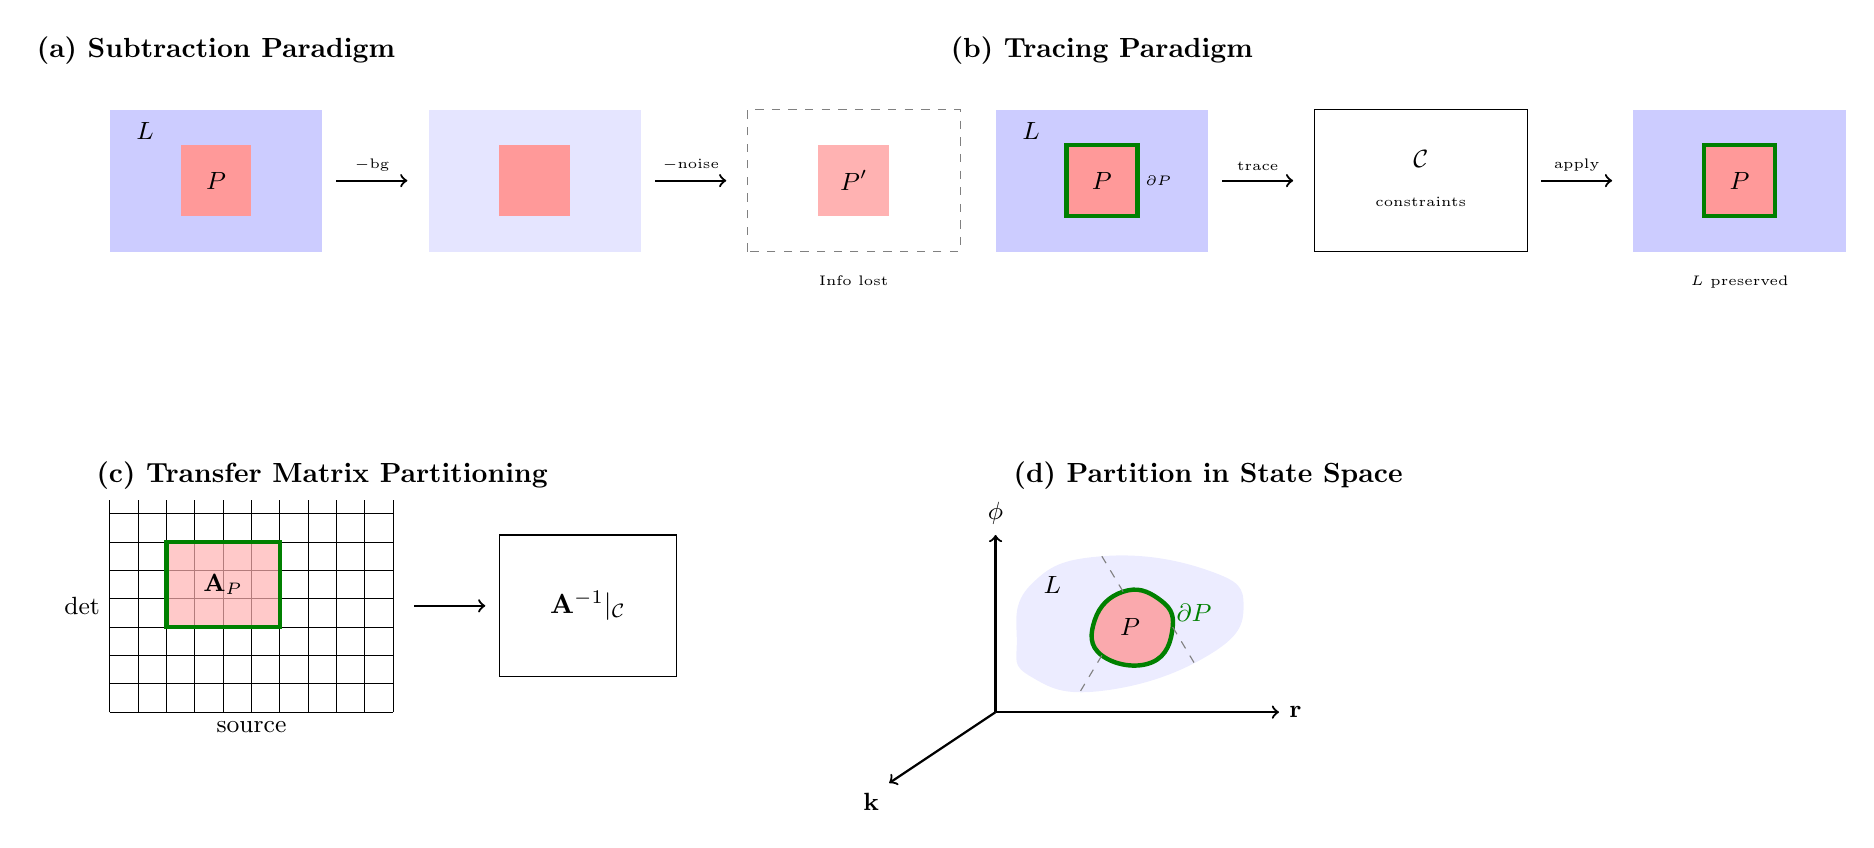
\begin{tikzpicture}[scale=0.9]
% Panel (a): Traditional Subtraction - top left
\begin{scope}[shift={(-4.5,3)}]
    \node[above] at (1.5,2.5) {\textbf{(a) Subtraction Paradigm}};
    % Full field
    \fill[blue!20] (0,0) rectangle (3,2);
    \fill[red!40] (1,0.5) rectangle (2,1.5);
    \node at (1.5,1) {\small $P$};
    \node at (0.5,1.7) {\small $L$};
    % Arrow
    \draw[->,thick] (3.2,1) -- (4.2,1);
    \node[above] at (3.7,1) {\tiny $-$bg};
    % After subtraction
    \begin{scope}[shift={(4.5,0)}]
        \fill[blue!10] (0,0) rectangle (3,2);
        \fill[red!40] (1,0.5) rectangle (2,1.5);
        \draw[->,thick] (3.2,1) -- (4.2,1);
        \node[above] at (3.7,1) {\tiny $-$noise};
    \end{scope}
    % Final
    \begin{scope}[shift={(9,0)}]
        \fill[white] (0,0) rectangle (3,2);
        \draw[gray,dashed] (0,0) rectangle (3,2);
        \fill[red!30] (1,0.5) rectangle (2,1.5);
        \node at (1.5,1) {\small $P'$};
        \node[below] at (1.5,-0.2) {\tiny Info lost};
    \end{scope}
\end{scope}

% Panel (b): Tracing Paradigm - top right
\begin{scope}[shift={(8,3)}]
    \node[above] at (1.5,2.5) {\textbf{(b) Tracing Paradigm}};
    % Full field with boundary traced
    \fill[blue!20] (0,0) rectangle (3,2);
    \fill[red!40] (1,0.5) rectangle (2,1.5);
    \draw[green!50!black,ultra thick] (1,0.5) rectangle (2,1.5);
    \node at (1.5,1) {\small $P$};
    \node at (2.3,1) {\tiny $\partial P$};
    \node at (0.5,1.7) {\small $L$};
    % Arrow
    \draw[->,thick] (3.2,1) -- (4.2,1);
    \node[above] at (3.7,1) {\tiny trace};
    % Constraint set
    \begin{scope}[shift={(4.5,0)}]
        \draw (0,0) rectangle (3,2);
        \node at (1.5,1.3) {\small $\mathcal{C}$};
        \node at (1.5,0.7) {\tiny constraints};
        \draw[->,thick] (3.2,1) -- (4.2,1);
        \node[above] at (3.7,1) {\tiny apply};
    \end{scope}
    % Reconstructed
    \begin{scope}[shift={(9,0)}]
        \fill[blue!20] (0,0) rectangle (3,2);
        \fill[red!40] (1,0.5) rectangle (2,1.5);
        \draw[green!50!black,ultra thick] (1,0.5) rectangle (2,1.5);
        \node at (1.5,1) {\small $P$};
        \node[below] at (1.5,-0.2) {\tiny $L$ preserved};
    \end{scope}
\end{scope}

% Panel (c): Transfer Matrix - bottom left
\begin{scope}[shift={(-4.5,-3.5)}]
    \node[above] at (3,3) {\textbf{(c) Transfer Matrix Partitioning}};
    % Matrix grid
    \draw[step=0.4] (0,0) grid (4,3);
    % Highlight partition
    \fill[red!30,opacity=0.7] (0.8,1.2) rectangle (2.4,2.4);
    \draw[green!50!black,ultra thick] (0.8,1.2) rectangle (2.4,2.4);
    % Labels
    \node[left] at (0,1.5) {\small det};
    \node[below] at (2,0) {\small source};
    \node at (1.6,1.8) {\small $\mathbf{A}_P$};
    % Arrow to constrained inverse
    \draw[->,thick] (4.3,1.5) -- (5.3,1.5);
    \begin{scope}[shift={(5.5,0)}]
        \draw (0,0.5) rectangle (2.5,2.5);
        \node at (1.25,1.5) {$\mathbf{A}^{-1}|_{\mathcal{C}}$};
    \end{scope}
\end{scope}

% Panel (d): 3D State Space - bottom right
\begin{scope}[shift={(8,-3.5)}]
    \node[above] at (3,3) {\textbf{(d) Partition in State Space}};
    % 3D axes
    \draw[->,thick] (0,0) -- (4,0) node[right] {\small $\mathbf{r}$};
    \draw[->,thick] (0,0) -- (0,2.5) node[above] {\small $\phi$};
    \draw[->,thick] (0,0) -- (-1.5,-1) node[below left] {\small $\mathbf{k}$};
    % 3D blob representing full state space
    \fill[blue!15,opacity=0.5] plot[smooth cycle,tension=0.8] coordinates {(0.5,0.5) (1.5,0.3) (3,0.8) (3.5,1.5) (3,2) (1.5,2.2) (0.5,1.8) (0.3,1)};
    % Partition subset
    \fill[red!40,opacity=0.8] plot[smooth cycle,tension=0.8] coordinates {(1.5,0.8) (2.2,0.7) (2.5,1.2) (2.3,1.6) (1.8,1.7) (1.4,1.3)};
    % Boundary membrane
    \draw[green!50!black,ultra thick] plot[smooth cycle,tension=0.8] coordinates {(1.5,0.8) (2.2,0.7) (2.5,1.2) (2.3,1.6) (1.8,1.7) (1.4,1.3)};
    % Labels
    \node at (0.8,1.8) {\small $L$};
    \node at (1.9,1.2) {\small $P$};
    \node[green!50!black] at (2.8,1.4) {\small $\partial P$};
    % Depth lines for 3D effect
    \draw[gray,dashed] (1.5,0.8) -- (1.2,0.3);
    \draw[gray,dashed] (2.5,1.2) -- (2.8,0.7);
    \draw[gray,dashed] (1.8,1.7) -- (1.5,2.2);
\end{scope}
\end{tikzpicture}
\caption{Panel comparison of imaging paradigms. (a) Traditional subtraction progressively destroys information through sequential filtering. (b) Boundary tracing identifies the partition through constraints, preserving the total field. (c) The transfer matrix contains all path information; partition extraction identifies the relevant submatrix through constraints. (d) Three-dimensional state space representation: the partition $P$ exists within the total field $L$, defined by its boundary membrane $\partial P$ in $(\mathbf{r}, \mathbf{k}, \phi)$ space.}
\label{fig:paradigm_comparison}
\end{figure}

\section{Discussion}

\subsection{Relationship to Existing Techniques}

RPI shares conceptual elements with:
\begin{itemize}
    \item \textbf{Computational photography}: Both invert optical transformations computationally
    \item \textbf{Wavefront sensing}: Both characterize optical transfer functions
    \item \textbf{Time-reversal acoustics}: Both exploit invertibility of wave equations
\end{itemize}

The distinctive contribution is the discrete combinatorial formulation enabling constraint-based reasoning.

\subsection{Fundamental vs. Practical Limits}

The RPI framework separates fundamental from practical limitations:
\begin{itemize}
    \item \textbf{Fundamental}: Photon number, detector noise
    \item \textbf{Not fundamental}: Aberrations, scattering, diffraction limit
\end{itemize}

Phenomena traditionally viewed as ``fundamental limits'' (diffraction) become computational problems solvable given sufficient information.

\subsection{Connection to Categorical Imaging}

RPI connects to the categorical partition framework \cite{partition2024}. Photon states form a category, optical elements are functors, and image reconstruction is computing inverse morphisms. The discrete path space is the morphism set between source and detector objects.

\section{Conclusion}

Refraction Puzzle Imaging recasts optical image formation as discrete combinatorial constraint satisfaction. By discretizing light propagation at extreme temporal resolution, continuous wave optics becomes finite state machine dynamics. Image reconstruction transforms from solving continuous inverse problems to satisfying discrete constraints.

The framework predicts remarkable capabilities: imaging through arbitrary aberrations, reconstruction through scattering media, and resolution limited only by photon statistics. While the ultimate temporal discretization ($10^{-156}$~s) is experimentally inaccessible, practical implementations at attosecond scales already enable sub-wavelength imaging.

RPI represents a paradigm shift from optical correction to computational inversion, suggesting that the fundamental limits of imaging are informational rather than optical.

\section*{Acknowledgments}

The author acknowledges the broader categorical imaging framework within which this work is situated.

\bibliographystyle{plain}
\bibliography{references}

\end{document}
